\documentclass[12pt]{chmullighw}
\usepackage{tikz}
\usepackage{tikz-qtree}
\usepackage{algorithm2e}
\usetikzlibrary{shapes,chains,fit,shapes,matrix}


% info for header block in upper right hand corner
\name{Chris Mulligan}
\uni{clm2186}
\class{COMS3137 Data Structures \& Algorithms}
\professor{Hershkop}
\assignment{Theory 4}
\duedate{November 14, 2013, \hspace{1em}  2 Days Late}

\lstset{language=Java, numbers=none, frame=l, captionpos=n}
\begin{document}
\problemlist{Theory 4} %Give us a nice big title
\begin{enumerate}

\item I interpret this question to mean there are $N$ individuals, numbered
$ i = 1, \ldots, N$. They each have $m_i$ miles, for a total of
$M = \sum_{j=1}^{N}m_i$ miles. They want to reward the $\log N$ individuals 
with the most miles.

A maxheap of the fliers can be built in \BigO{N} time, sorted by number of accumulated miles. Then we need to pull out the $\log N$ largest individuals, which costs \BigO{\log N} each time, for a total removal runtime of \BigO{\log N\cdot \log N}. Because the removal runtime is dominated by the linear runtime, the overall the runtime is \BigO{N + \log N \cdot \log N} = \BigO{N}.


\item A priority queue based on an array is a heap. Insert is \BigO{\log n}. You insert the node in the next available spot, and then perform a "bubble up" of the node in order to satisfy the heap parameter. Because the tree is at most $\log n$ high, the number of comparisons and swaps is at most \BigO{\log n}.

Assuming this is a minheap, and that findmin returns and removes the minimum node, the runtime is also \BigO{\log n}. The minimum node will always be the root, so finding it is \BigO{1}. However once we remove it, we have to bubble down the empty space to maintain the heap ordering, which will cost at most the height of the tree, \BigO{\log n}. Thus the overall runtime for findmin is \BigO{\log n}.


\item We can use a similar approach as quicksort or other methods that use a pivot. We put two pointers at the beginning and end of the array. We advance each towards the middle as long as the element it's pointing to is the correct color. If it's not correct (eg the left pointer is pointing to a red element), wait until both are incorrect, then swap the two. Those two elements will then be on the correct side, and we continue each pointer. Once the pointers meet, we know the array is sorted such that all blue elements are before all red elements. The runtime is simply \BigO{n} because it is complete after a single pass of checking every element.

The most computationally simple method of extending to 3 colors is to make this a two pass algorithm. In the first pass you combine two colors, for example blue and green, and treat them as one color. That will separate the blue/green elements from the red elements. Then you call the same algorithm on the blue/green section to separate those two colors. This can extend to arbitrary numbers of colors, but will become very inefficient. The runtime will be \BigO{cn} where $c$ is the number of colors we wish to separate.


\item We can create a hash table, and add each element to the hash table. If the element collides, we can check to see if it's an exact match, or just a hash collision. Adding each element should take \BigO{1}, for an overall runtime of \BigO{n}. You can iterate over the hash table to list the unique elements.

\item {\em Note: links above are left to right, links below are from right to left}

\begin{enumerate} \renewcommand{\labelenumii}{\alph{enumii}.}
    \item union(x, y) makes y the child of x:

        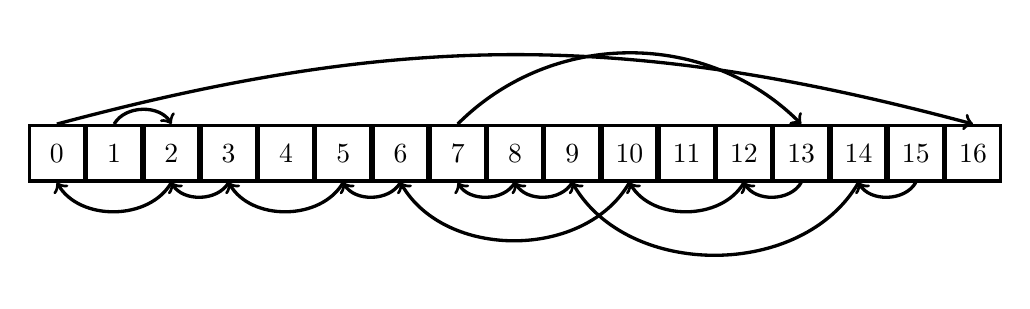
\begin{tikzpicture}
        \tikzstyle{every path}=[very thick]

        \edef\sizetape{.7cm}
        \tikzstyle{ht}=[draw,minimum size=\sizetape]
        \tikzstyle{num}=[draw=none]
        \tikzstyle{value}=[draw]

        \begin{scope}[start chain=1 going right,node distance=-0.15mm]
        \foreach \x in {0, 1,...,16} {
            \node [on chain=1,ht] (\x) {};
            \node [num] at (\x.center) (\x_label) {$\x$};
        };
        \end{scope}

        \draw[->, bend left=60] (15.south) to (14.south);   % 15->14
        \draw[->, bend left=60] (13.south) to (12.south);   % 13->12
        \draw[->, bend left=60] (14.south) to (9.south);    % 15->9
        \draw[->, bend left=60] (12.south) to (10.south);   % 13->10
        \draw[->, bend left=60] (8.south) to (7.south);     % 8->7
        \draw[->, bend left=60] (9.south) to (8.south);     % 15->8
        \draw[->, bend left=60] (10.south) to (6.south);    % 13->6
        \draw[->, bend left=60] (6.south) to (5.south);    % 13->5
        \draw[->, bend left=60] (5.south) to (3.south);    % 13->3
        \draw[->, bend left=60] (1.north) to (2.north);    % 1->2
        \draw[->, bend left=15] (0.north) to (16.north);    % 0->16
        \draw[->, bend left=60] (2.south) to (0.south);    % 2->0
        \draw[->, bend left=45] (7.north) to (13.north);    % 15->13
        \draw[->, bend left=60] (3.south) to (2.south);    % 15->2
        
        \end{tikzpicture}

\item union by height:

        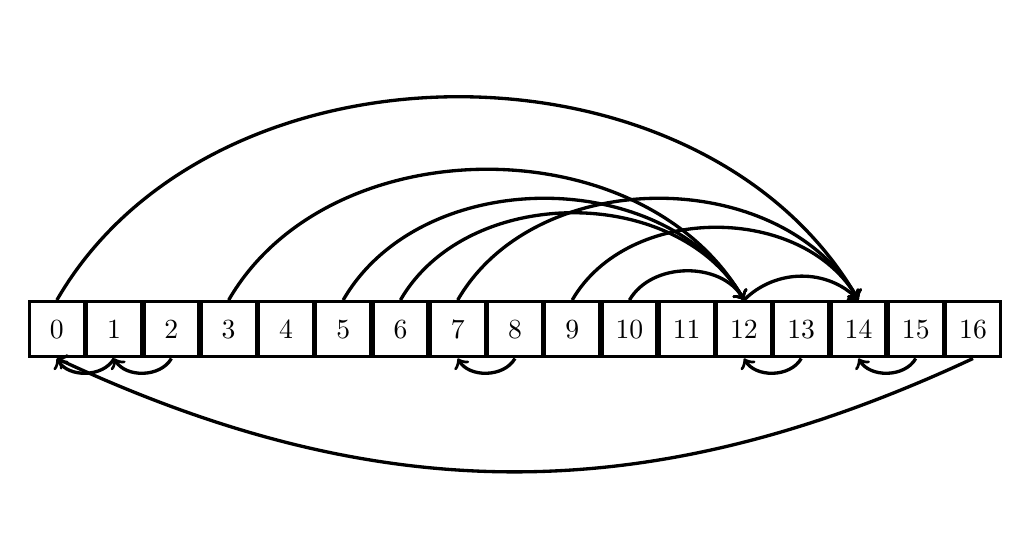
\begin{tikzpicture}
        \tikzstyle{every path}=[very thick]

        \edef\sizetape{.7cm}
        \tikzstyle{ht}=[draw,minimum size=\sizetape]
        \tikzstyle{num}=[draw=none]
        \tikzstyle{value}=[draw]

        \begin{scope}[start chain=1 going right,node distance=-0.15mm]
        \foreach \x in {0, 1,...,16} {
            \node [on chain=1,ht] (\x) {};
            \node [num] at (\x.center) (\x_label) {$\x$};
        };
        \end{scope}

        \draw[->, bend left=60] (15.south) to (14.south);   % 15->14
        \draw[->, bend left=60] (13.south) to (12.south);   % 13->12
        \draw[->, bend left=60] (9.north) to (14.north);    % 15->9
        \draw[->, bend left=60] (10.north) to (12.north);   % 13->10
        \draw[->, bend left=60] (8.south) to (7.south);     % 8->7
        \draw[->, bend left=60] (7.north) to (14.north);     % 15->8
        \draw[->, bend left=60] (6.north) to (12.north);    % 13->6
        \draw[->, bend left=60] (5.north) to (12.north);    % 13->5
        \draw[->, bend left=60] (3.north) to (12.north);    % 13->3
        \draw[->, bend left=60] (2.south) to (1.south);    % 1->2
        \draw[->, bend left=25] (16.south) to (0.south);    % 0->16
        \draw[->, bend left=60] (1.south) to (0.south);    % 2->0
        \draw[->, bend left=45] (12.north) to (14.north);    % 15->13
        \draw[->, bend left=60] (0.north) to (14.north);    % 15->2
        
        \end{tikzpicture}

    \item union by size:

        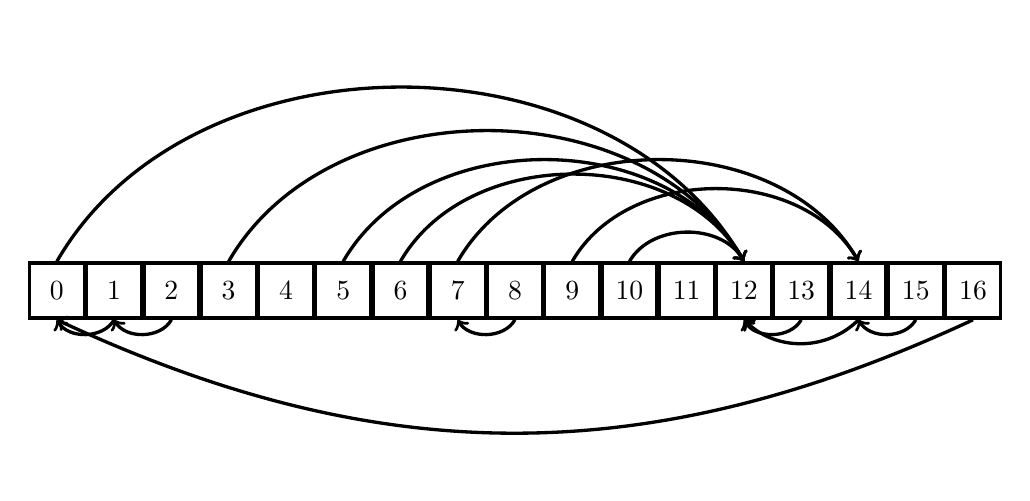
\begin{tikzpicture}
        \tikzstyle{every path}=[very thick]

        \edef\sizetape{.7cm}
        \tikzstyle{ht}=[draw,minimum size=\sizetape]
        \tikzstyle{num}=[draw=none]
        \tikzstyle{value}=[draw]

        \begin{scope}[start chain=1 going right,node distance=-0.15mm]
        \foreach \x in {0, 1,...,16} {
            \node [on chain=1,ht] (\x) {};
            \node [num] at (\x.center) (\x_label) {$\x$};
        };
        \end{scope}

        \draw[->, bend left=60] (15.south) to (14.south);   % 15->14
        \draw[->, bend left=60] (13.south) to (12.south);   % 13->12
        \draw[->, bend left=60] (9.north) to (14.north);    % 15->9
        \draw[->, bend left=60] (10.north) to (12.north);   % 13->10
        \draw[->, bend left=60] (8.south) to (7.south);     % 8->7
        \draw[->, bend left=60] (7.north) to (14.north);     % 15->8
        \draw[->, bend left=60] (6.north) to (12.north);    % 13->6
        \draw[->, bend left=60] (5.north) to (12.north);    % 13->5
        \draw[->, bend left=60] (3.north) to (12.north);    % 13->3
        \draw[->, bend left=60] (2.south) to (1.south);    % 1->2
        \draw[->, bend left=25] (16.south) to (0.south);    % 0->16
        \draw[->, bend left=60] (1.south) to (0.south);    % 2->0
        \draw[->, bend left=45] (14.south) to (12.south);    % 15->13
        \draw[->, bend left=60] (0.north) to (12.north);    % 15->2
        
        \end{tikzpicture}


\end{enumerate}

\item One of the (many) disadvantages of bubble sort is that small elements at the end take a very long time to move to the beginning, requiring each element to swap with it. By alternating reverse passes Hubble Sort can quickly move these small elements towards the front. This does not change the big-O runtime of the algorithm from \BigO{n^2}, but it may be slightly faster in a practical sense by avoiding certain worst case scenarios. On modern computers it may also have slightly  better than expected performance due decreased cache misses.

\end{enumerate} %end of questions
\end{document}
